%%%%%%%%%%%%%%%%%%%%%%%%%%%%%%%%%%%%%%%%%%%
\subsection{Концептуальная постановка задачи}
%%%%%%%%%%%%%%%%%%%%%%%%%%%%%%%%%%%%%%%%%%%
\begin{frame}%[allowframebreaks=0.9,t]

\begin{block}{Объект исследований}
\textexample{\ObjectOfResearch}
\end{block}

\begin{block}{Цель исследования}
\textexample{\GoalOfResearch}
\end{block}

\begin{block}{Задачи исследования}
\begin{enumerate}
	\arrowitem{Сравнить подходы к реализации графоориентированного подхода к решению задач проектирования на примере нескольких существующих программных комплексов}
	\arrowitem{Исследовать программную структуру модуля каркаса GBSE, отвечающего за струкутуру графовых моделей}
	\arrowitem{Определить требования к структуре данного модуля}
	\arrowitem{Разработать новую структуру, которая бы отвечала сформулированным требованиям}
\end{enumerate}
\end{block}

\end{frame}

%%%%%%%%%%%%%%%%%%%%%%%%%%%%%%%%%%%%%%%%%%%
\subsection{Формирование требовний к графовым моделям}
%%%%%%%%%%%%%%%%%%%%%%%%%%%%%%%%%%%%%%%%%%%
\begin{frame}%[allowframebreaks=0.9,t]
	\begin{figure}
		\centering
		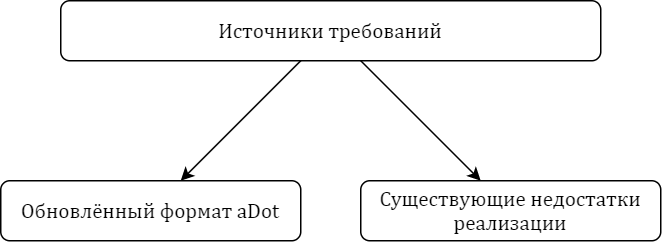
\includegraphics[width=\textwidth]{images/requirement_sources.png}
		\caption{}
		\label{fig:requirementSources}
	\end{figure}
\end{frame}
%%%%%%%%%%%%%%%%%%%%%%%%%%%%%%%%%%%%%%%%%%%
\subsection{Требования формата aDot}
%%%%%%%%%%%%%%%%%%%%%%%%%%%%%%%%%%%%%%%%%%%
\begin{frame}%[allowframebreaks=0.9,t
	\begin{figure}
		\centering
		\includegraphics[width=\textwidth]{images/new_structure_example.png}
		\caption{Пример графовой модели с новой структурой c пояснениями}
	\end{figure}
\end{frame}
%%%%%%%%%%%%%%%%%%%%%%%%%%%%%%%%%%%%%%%%%%%
\subsection{Недостатки текущей реализации}
%%%%%%%%%%%%%%%%%%%%%%%%%%%%%%%%%%%%%%%%%%%
\begin{frame}
	\begin{figure}
			\centering
			\includegraphics[width=\textwidth]{images/new_structure_example.png}
			\caption{Пример графовой модели в текущем формате}
	\end{figure}
\end{frame}

\begin{frame}
	\begin{figure}
		\centering
		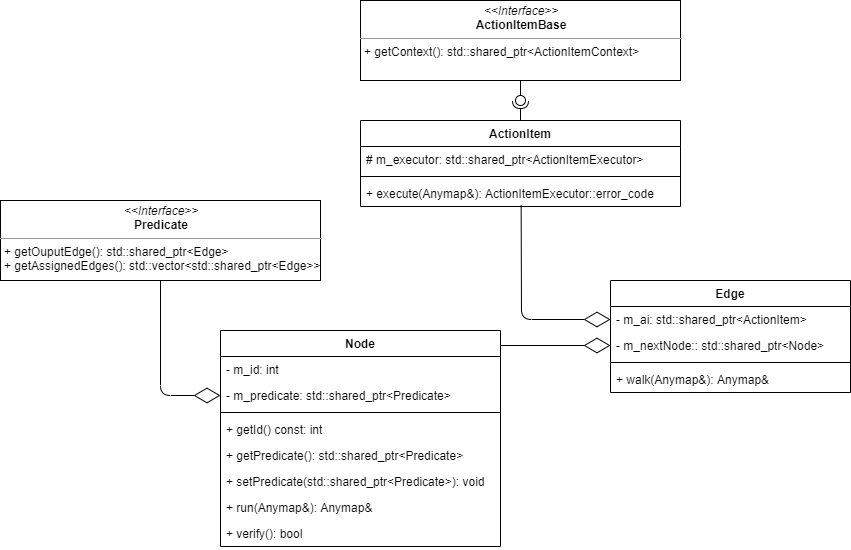
\includegraphics[width=\textwidth]{images/structure.png}
		\caption{Текущая структура классов, связанных с графовыми моделями}
	\end{figure}
\end{frame}

